\documentclass[12pt,a4paper,openright,twoside]{book}
\usepackage[utf8]{inputenc}
\usepackage{disi-thesis}
\usepackage{code-lstlistings}
\usepackage{notes}
\usepackage{shortcuts}
\usepackage{acronym}
\usepackage{hyperref} % links
\usepackage{comment} % for multi-line comments
\usepackage{booktabs} % for better tables
\usepackage{xcolor}
\usepackage{listings}
\usepackage{caption}
\usepackage{subcaption}
\usepackage{svg}

\showboxdepth=5
\showboxbreadth=5

\school{\unibo}
\programme{Corso di Laurea Magistrale in Ingegneria e Scienze Informatiche}
\title{Fancy Title}
\author{Penazzi Paolo}
\date{\today}
\subject{Supervisor's course name}
\supervisor{Prof. Supervisor Here}
\cosupervisor{Prof. CoSupervisor 1}
\session{III}
\academicyear{2022-2023}

% Definition of acronyms
\acrodef{CAS}{Collective Adaptive Systems}
\acrodef{vm}[VM]{Virtual Machine}
\acrodef{SUT}{System Under Test}


\mainlinespacing{1.241} % line spacing in main matter, comment to default (1)

\begin{document}

\frontmatter\frontispiece

\begin{abstract}	
Max 2000 characters, strict.
\end{abstract}

%----------------------------------------------------------------------------------------
\tableofcontents   
\listoffigures     % (optional) comment if empty
\lstlistoflistings % (optional) comment if empty
%----------------------------------------------------------------------------------------

\mainmatter

%----------------------------------------------------------------------------------------
\chapter{Introduction}
\label{chap:introduction}
%----------------------------------------------------------------------------------------

\paragraph{Motivation}

\paragraph{Objectives}

\paragraph{Thesis Structure}

%----------------------------------------------------------------------------------------
\chapter{Background}
%----------------------------------------------------------------------------------------

\section{Collective Adaptive Systems}

\ac{CAS} are a complex type of distributed network, composed of a large number of heterogeneous entities.
The two main characteristics that distinguish these systems are the ability to adapt their behavior to dynamically changing open-ended environments
and the pursuit of a collective goal, achieved through interaction without specific external or internal central control. \cite{DBLP:series/lncs/HolzlRW08, DBLP:journals/corr/abs-1108-5643}
It is important to note that \ac{CAS} can be composed of heterogeneous entities, each with its capabilities and goals.
To achieve the collective goal without central control, \ac{CAS} often adopts cooperative operating strategies to run distributed decision-making mechanisms. \cite{DBLP:journals/tomacs/Aldini18} \\

Nowadays, many systems are adaptive and collective: drone swarms tasked with monitoring an area, 
wearable devices to manage crowd congestion during a public event, cars on streets connected to handle traffic, 
are all examples of CAS. \cite{DBLP:journals/sttt/NicolaJW20}

\begin{figure*}[ht]
  \centering
  \begin{subfigure}[b]{0.49\textwidth}
      \centering
      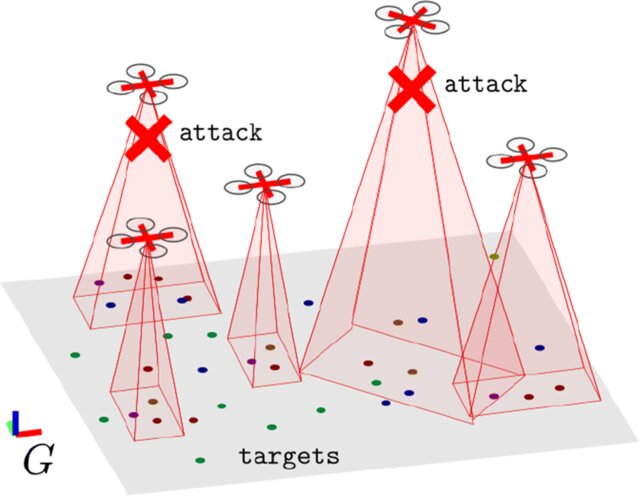
\includegraphics[width=0.9\textwidth]{figures/swarm2.jpeg}
  \end{subfigure}

  \begin{subfigure}[b]{0.49\textwidth}
      \centering
      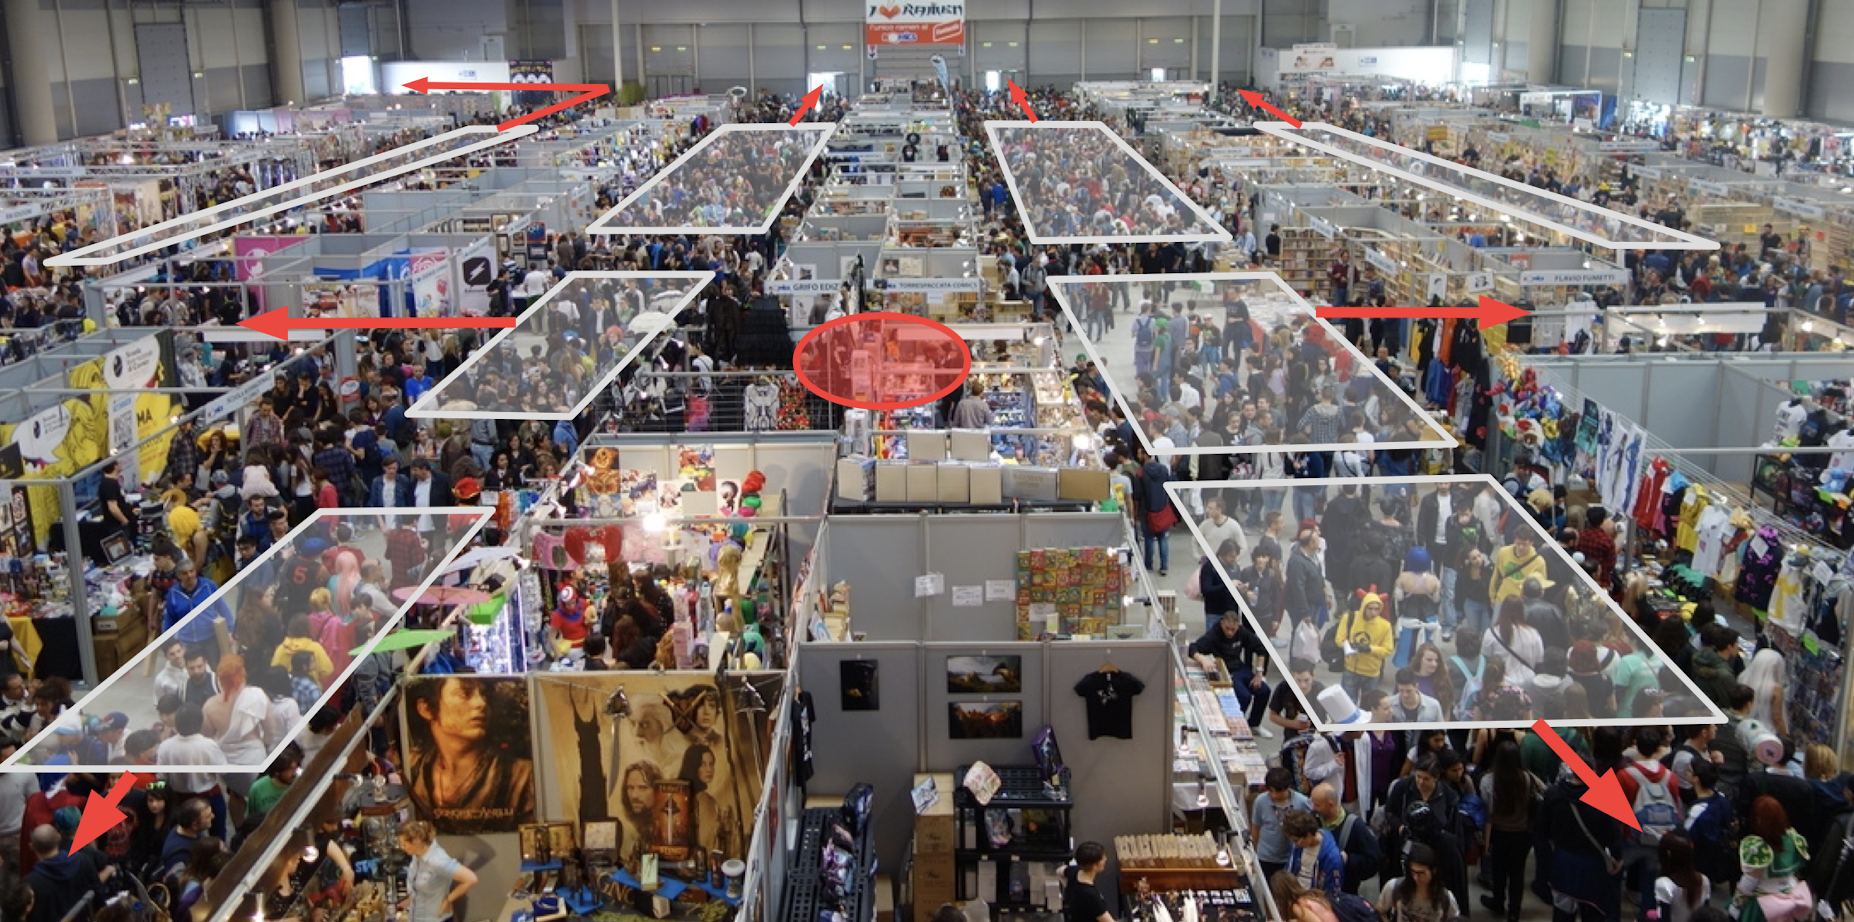
\includegraphics[width=0.8\textwidth]{figures/crowd.png}
  \end{subfigure}
  \caption{Some examples of CAS.}
\end{figure*}

\section{Aggregate Programming}

In recent years, we have witnessed a shift in the production of computing devices: moving from a few large and powerful devices to a large number of small and lightweight devices. 
There is often talk about the Internet of Things and how technology has become pervasive, impacting every aspect of our lives with electronic devices.
This trend has led to a change in the way we compute data: no longer focusing on a single machine performing heavy computation, but rather on a distributed network of devices communicating and collaborating to achieve a result. 
Computation is thus divided and distributed across various devices in the network. 
This has introduced an additional level of complexity in programming these systems as it is necessary to consider issues such as communication between devices, 
concurrency, or failures. Furthermore, as these systems grow in complexity, it becomes challenging to create solutions that are extensible, modular, and easily testable. \cite{DBLP:conf/ecoop/CasadeiV16} \\

Aggregate programming is a new approach to developing complex distributed systems that abstract from individual devices, focusing on programming the collective. 
Through a layer that handles and hides some problematic aspects of these networks, such as communication between devices and details of individual entities, 
it is possible to simplify the design and maintenance of these systems. \cite{DBLP:journals/computer/BealPV15, DBLP:conf/sfm/BealV16} \\

Aggregate programming is based on the concept of a computational field, which is a global map associating each device in the network with its local value, 
and on that of field calculus, a minimal core that provides basic constructs for working with fields. \cite{DBLP:journals/corr/ViroliADPB16}

\section{Simulation}

In computer science, simulation is the process of executing software in a controlled environment to evaluate its behavior. 
Simulations can be used to test the correctness of a program, evaluate its performance, or understand its behavior in a specific scenario. 
The key point of a simulation is to execute the software under controlled and repeatable conditions to compare different executions. 
This cannot be done without a simulator, which provides the user with all the tools needed to run the simulation. \cite{argun2021simulation, bagrodia1998parsec} \\
The importance of simulators becomes clear when testing \ac{CAS}. 
It is not feasible to create a real environment, such as a network of 100 drones or a crowd of 1000 people, to test a program.
Simulators allow us to create a virtual environment where we can run the program and evaluate its behavior. \\

\section{Alchemist}

The reference simulator for this work is Alchemist. \cite{Pianini_2013}
Alchemist is a meta-simulator, open-source, for simulating complex distributed systems. It is termed a meta-simulator because it is based on generic abstractions. 
The meta-model of Alchemist is inspired by biochemistry and consists of various entities:
\begin{itemize}
  \item \textbf{Molecule} The name of a data item.
  \item \textbf{Concentration} The value associated with a molecule.
  \item \textbf{Node} A container of molecules and concentrations. Disposed inside the environment.
  \item \textbf{Environment} The abstraction for the space. It contains nodes and can tell the position of a node in the space and the distance between two nodes.
  \item \textbf{Linking Rule} A rule that defines the relation between nodes.
  \item \textbf{Reaction} Events fired according to a time distribution and set of conditions.
  \item \textbf{Condition} A function that takes the current environment as input and outputs a boolean and a number. The output influences the execution of the corresponding reaction.
  \item \textbf{Action} Models a change in the environment.
\end{itemize}

Here is the visual representation of the Alchemist meta-model.

\begin{figure}[h]
  \centering
  \includegraphics[width=\textwidth]{figures/alchemist-model.png}
  \caption{Alchemist meta-model}
\end{figure}

\begin{figure}[h]
  \centering
  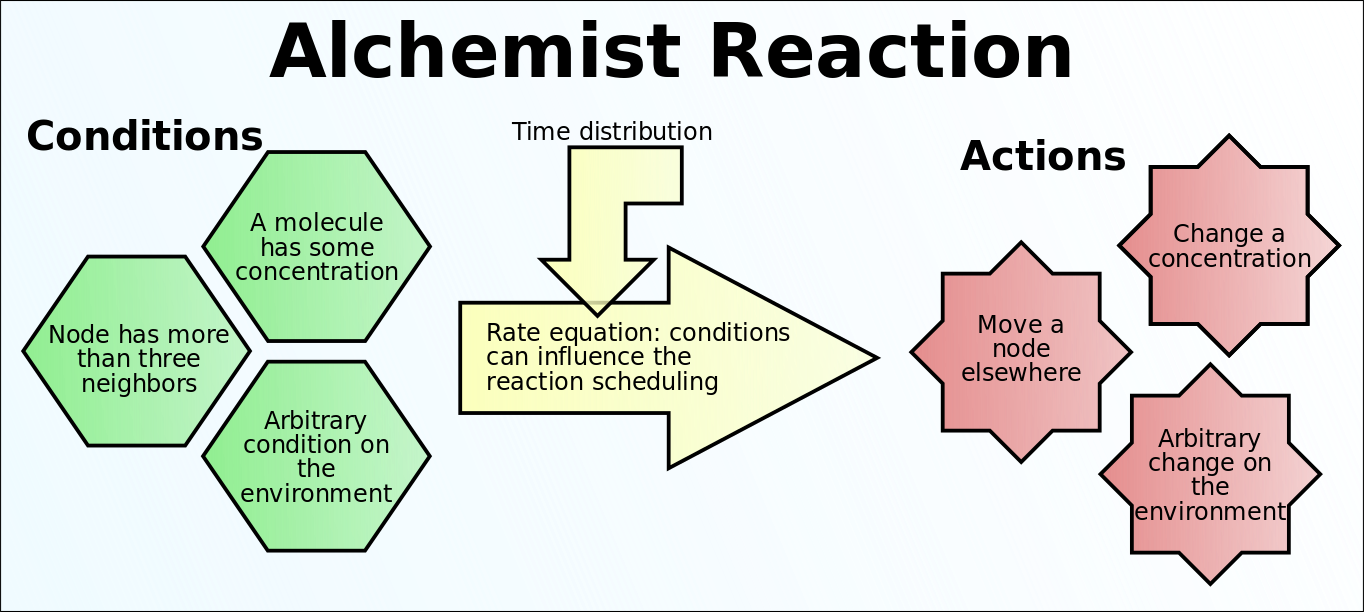
\includegraphics[width=\textwidth]{figures/alchemist-reaction.png}
  \caption{Alchemist reaction}
\end{figure}

The key of the Alchemist extensibility is the very generic interpretation of molecules and concentrations. An incarnation maps this generic chemical abstraction to a specific use case.
Alchemist supports four incarnations: 
SAPERE \cite{DBLP:conf/saso/CastelliMRZ11}, the first supported incarnation, based on the concept of Live Semantic Annotation (LSA), 
ScaFi \cite{DBLP:journals/softx/CasadeiVAP22}, which is a Scala-based library and framework for Aggregate Programming, 
Protelis \cite{DBLP:conf/sac/PianiniVB15}, a programming language for aggregate computing, and 
Biochemistry incarnation.

\begin{figure}[h]
  \centering
  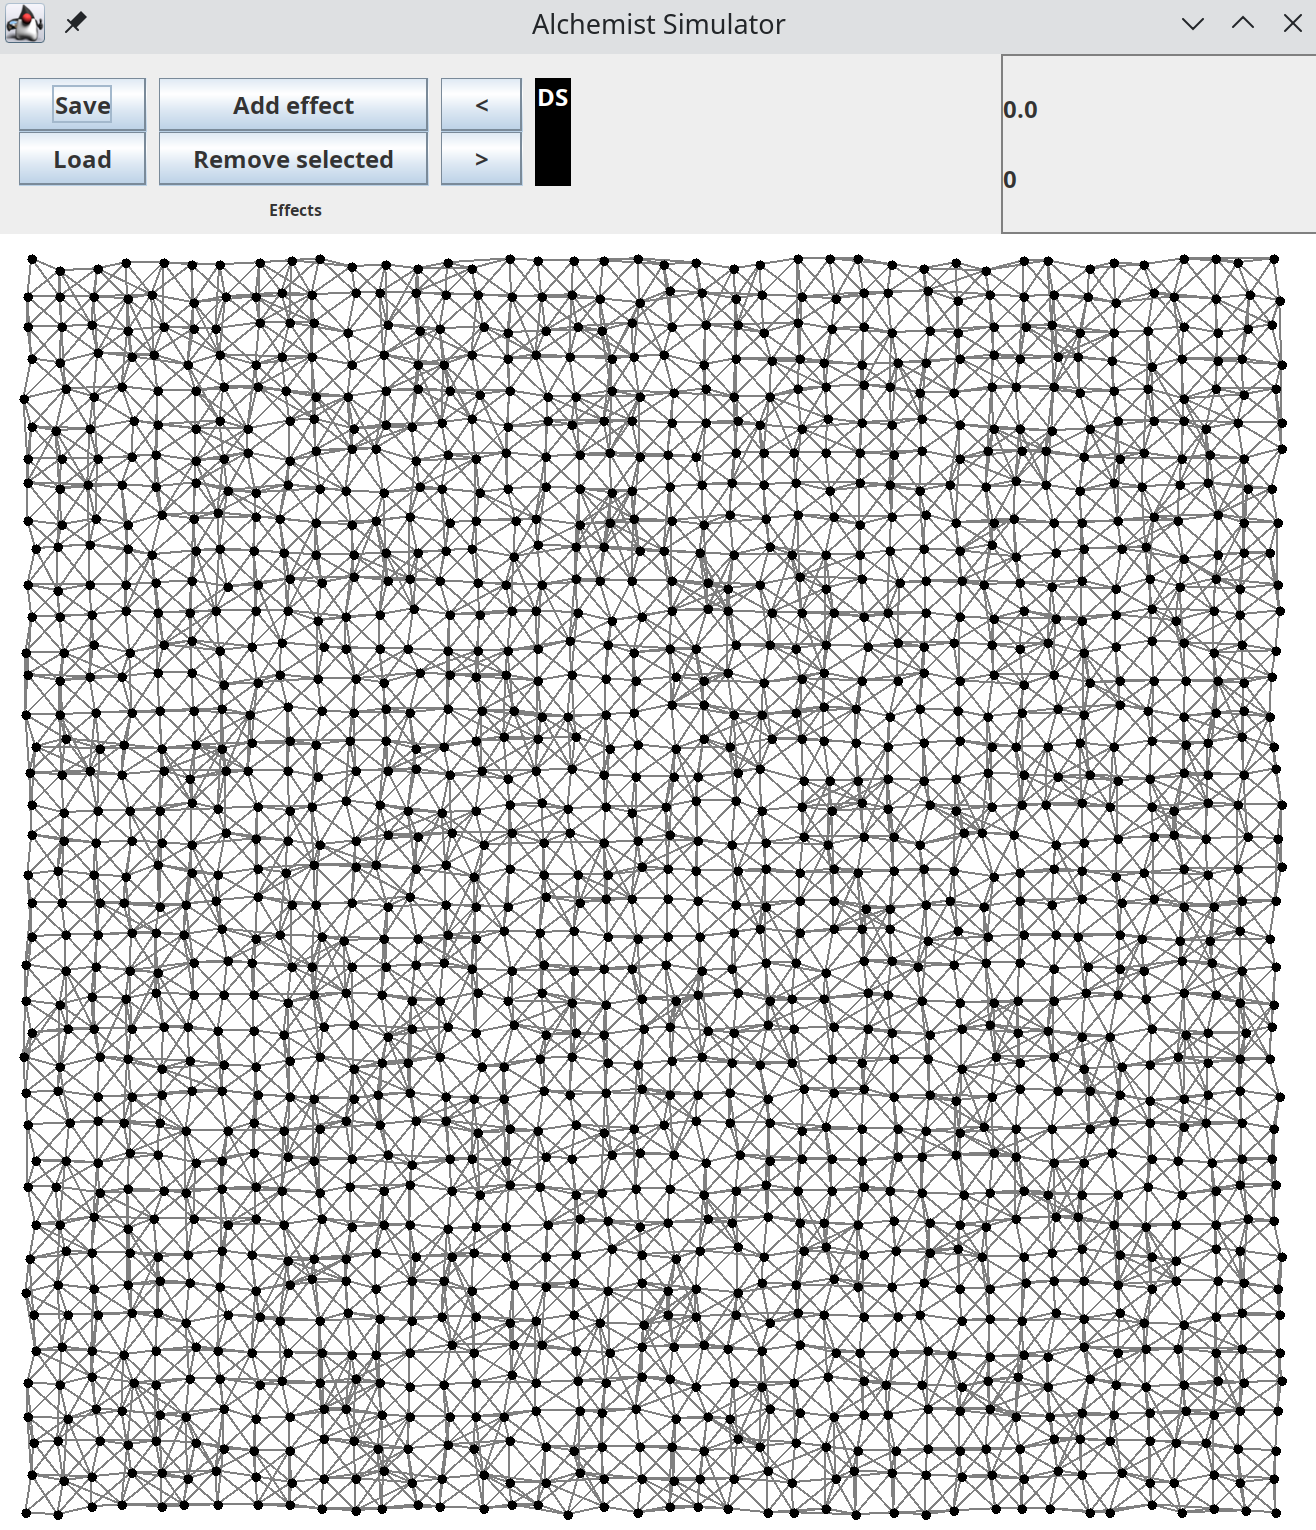
\includegraphics[width=\textwidth]{figures/alchemist.png}
  \caption{A grid of nodes in Alchemist}
\end{figure}

\section{Testing}

In every field of engineering, testing is a fundamental part of the development process.
Testing refers to the process carried out to verify and validate a system, according to its requirements. \cite{Spillner2011}

In every research field, It is important to evaluate the behavior of newly developed algorithms against state-of-the-art solutions.
This allows us to understand whether a newly developed solution is better than an existing one in a certain scenario.

Having a set of benchmarks available permits to do so: compare the \ac{SUT} against other solutions.

%----------------------------------------------------------------------------------------
\chapter{Requirements}
%----------------------------------------------------------------------------------------

\section*{Domain}

In the context of collective adaptive systems, there is a lack of a framework that allows the user to conduct a series of tests, utilizing different simulators, in a unified environment. 
The approach proposed in this work aims to create a framework that enables repeated testing on various simulators, process the results to evaluate and compare the solution.

A domain-driven approach was employed in the development. The choices made were based on the study of existing simulators and user needs. A Ubiquitous Language was defined, containing the key concepts of this domain and their definitions. 
These concepts were then utilized in the framework development and can be found in the implementation.

User Stories were also defined, helpful in understanding what users need and thus what features the framework should support.

\section{Ubiquitous Language}

To better understand the problem domain and to avoid misunderstandings, a ubiquitous language has been defined.

\begin{table}[h]
    \centering
    \begin{tabular}{|l|p{0.8\textwidth}|}
    \toprule
    \textbf{Term} & \textbf{Meaning} \\
    \midrule                                                                                                                                                              
    Testing & The overall process carried out to verify and validate a system, according to requirements, to promote the desired internal and external quality and to mitigate risks in development and products. \\ \hline
    Testbed & A platform for rigorous, transparent and replicable environment for experimentation and testing TODO Cite \\ \hline
    Solution & A set of algorithms leading to achieving goals and overcoming the problem posted \\ \hline
    Scenario & Contains all the information about the test execution: the simulation platform, the metrics, the input parameters \\ \hline
    Simulator & A software that allows the user to see how its program would behave in a real environment \\ \hline
    \end{tabular}
    \caption{Domain Ubiquitous Language}
    \end{table}

\section{User Stories}

\section{Requirements}

\begin{itemize}
  \item It must be easily extendable to allow the addition of other simulators without compromising the functionality of the already supported simulators.
  \item It should not limit the user in any way, allowing them to test what they want, to the extent that specific simulators permit.
  \item It should facilitate the user in testing collective adaptive systems.
\end{itemize}

%----------------------------------------------------------------------------------------
\chapter{Design}
%----------------------------------------------------------------------------------------

\section{Architecture}

At an abstract level, the testbed is a framework that allows the user to define a benchmark, that will be executed under the hood, before returning the results to the user.
The following image shows the abstract architecture of the testbed.

\begin{figure}[h]
  \centering
  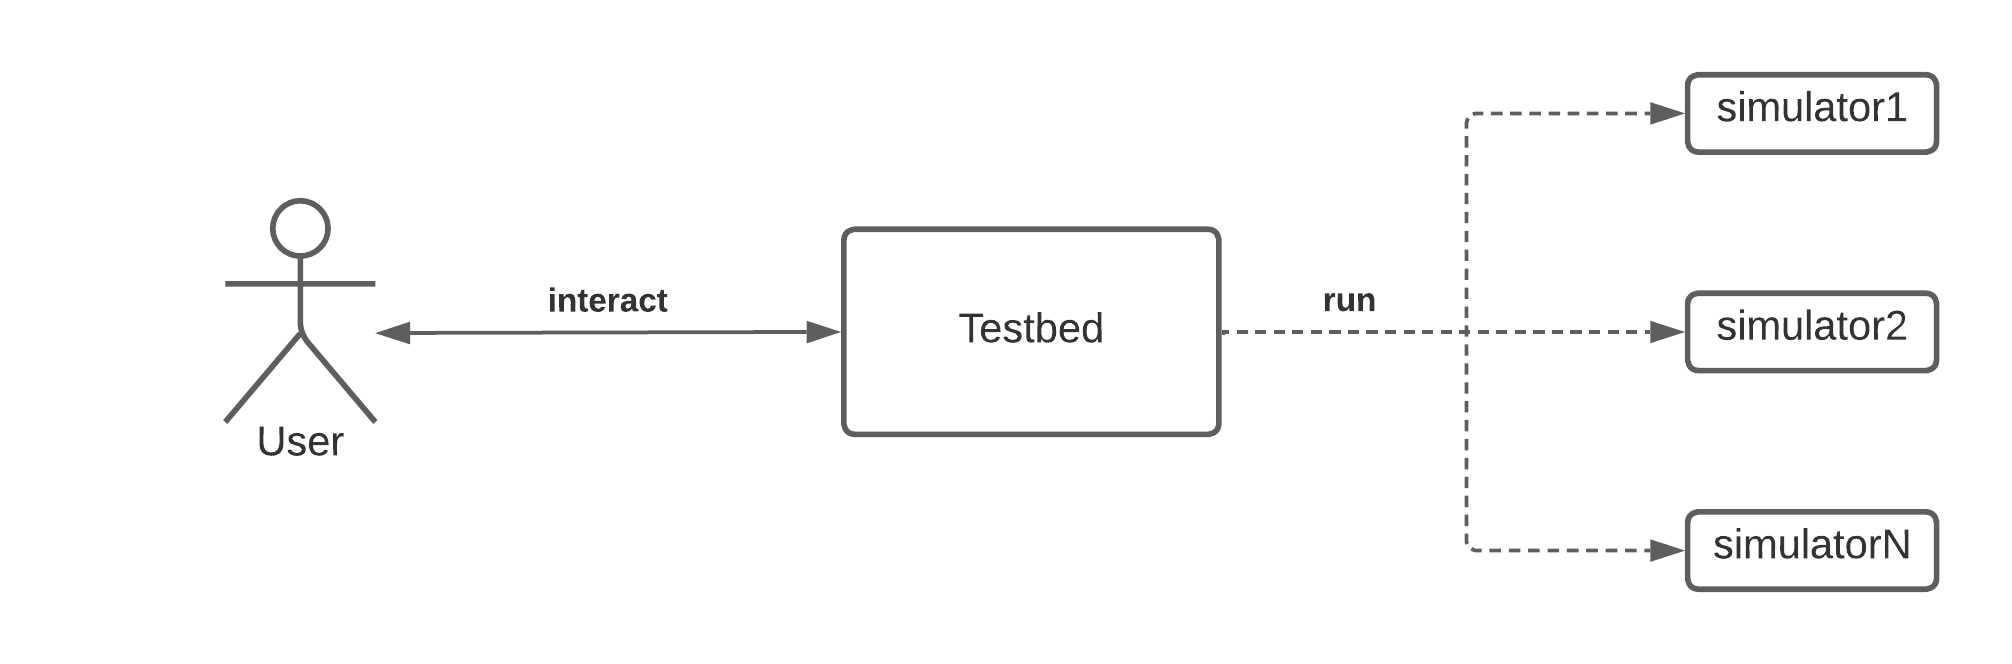
\includegraphics[width=\textwidth]{figures/architecture-high-level.png}
  \caption{Abstract architecture of the testbed}
\end{figure}

The Testbed is composed of different components, each with a specific role.
The main component is the Controller which is responsible for the entire execution of the benchmark. It takes in input a configuration file, which is forwarded, after a few integrity checks, to the Parser.
The Parser reads the input file and returns a benchmark model. The Benchmark Model is a representation of the input file, and it contains all the information needed to execute the benchmark.
The controller then creates and runs a specific Executor for each scenario to be executed. The Executor type depends on the simulator used in the scenario.
The executor handles the execution of the scenario, by launching the simulator with the correct parameters.
After each simulation is completed, a Listener is created to read the simulation output. The output is stored in a data structure inside the Testbed.
Once all the simulations are completed, the output is processed, and a view component is created to display the results to the user.

The following image shows the architecture of the system.

\begin{figure}[ht]
    \centering
    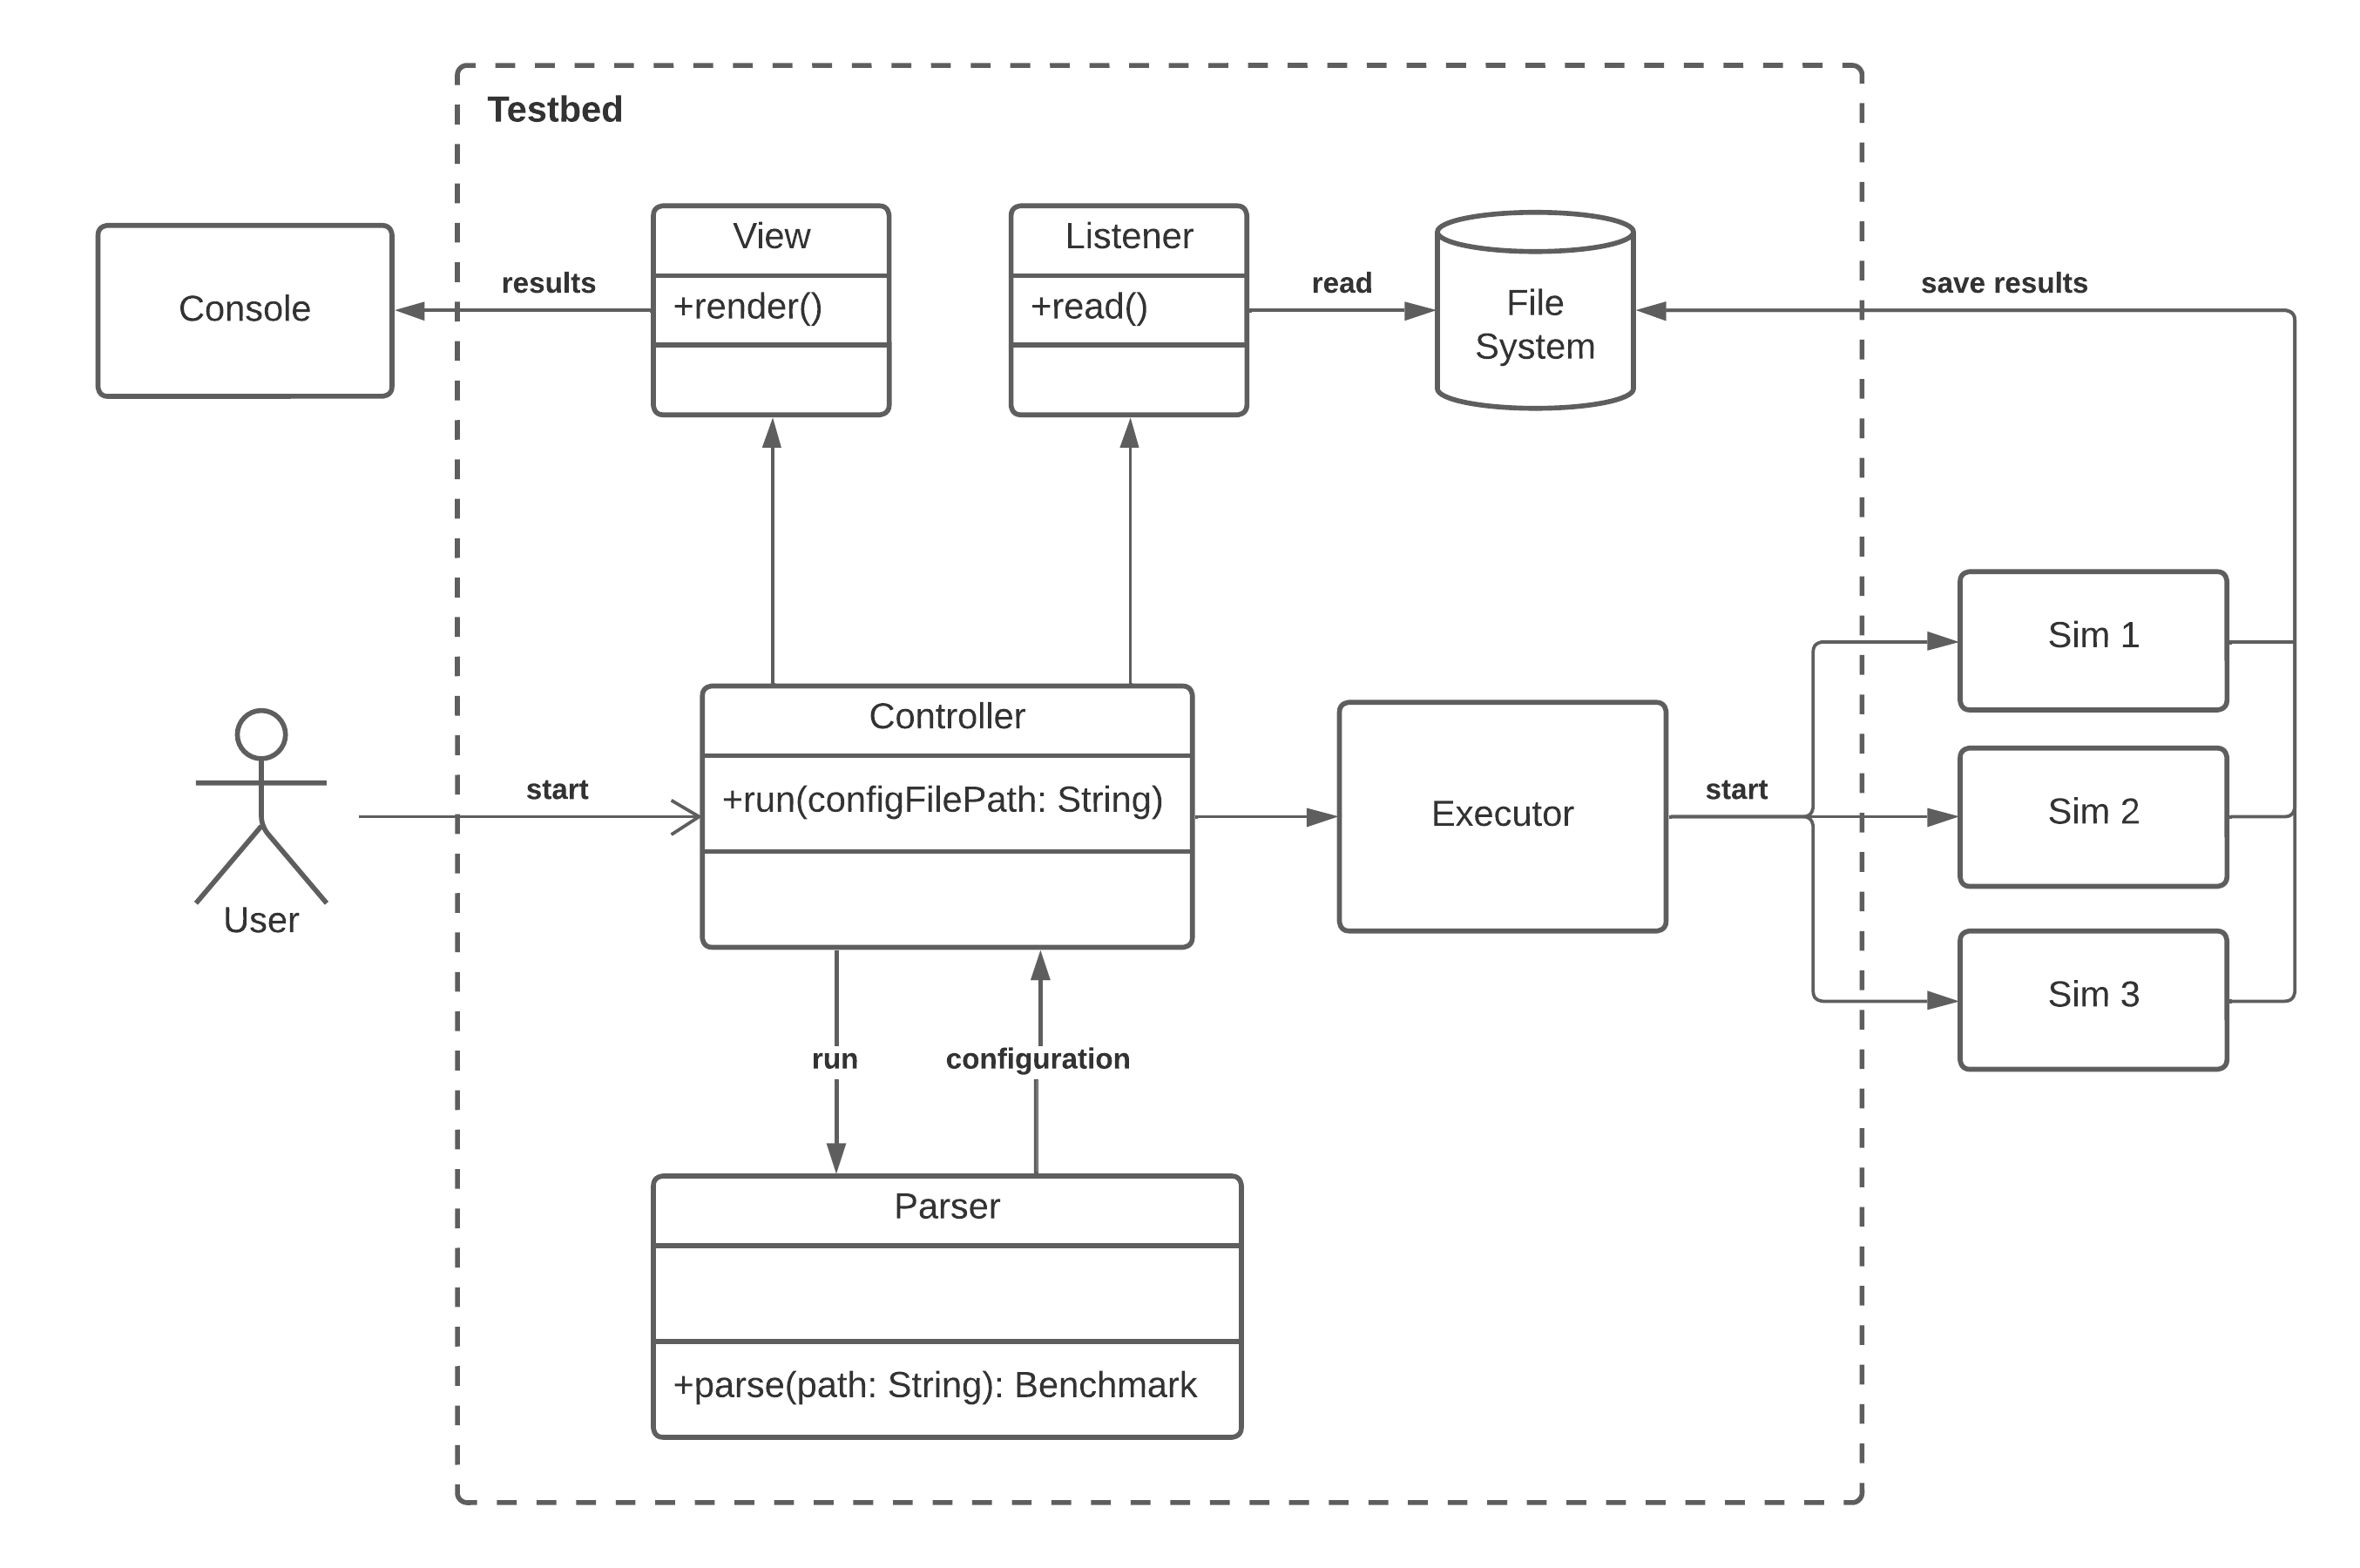
\includegraphics[width=\textwidth]{figures/testbed-architecture.png}
    \caption{Architecture of the system (v0.1)}
    \label{fig:random-image}
\end{figure}

The following diagram shows a detailed view of the benchmark execution.

\begin{figure}[ht]
  \centering
  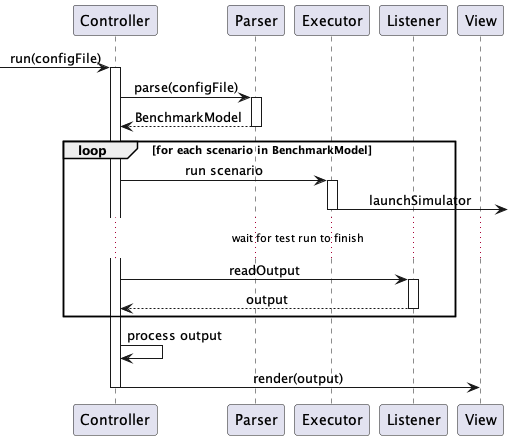
\includegraphics[width=\textwidth]{figures/execution-sequence-diagram.png}
  \caption{Architecture of the system (v0.1)}
  \label{fig:random-image}
\end{figure}

\subsection{Benchmark Model}

The benchmark model is the core of the system. It contains all the information about the benchmark execution.
Here is a brief description of the main classes.

\paragraph*{Strategy} The strategy section contains generic information about the testbed configuration. None of these 
are simulator-specific instructions.
All the keywords in this section are optional, and if not specified the default value is used: the execution will be
single-threaded and the execution order will be random.

\paragraph*{Simulators} The simulators section contains the configuration of each simulator used in the testbed.
Each simulator has a name, a version, and a list of scenarios. The name is mandatory, while the version is optional 
and is currently not used. The testbed will always use the latest version.

The scenario configuration is more complex, as each simulator has different ways to configure the scenario.
When adding support for a new simulator, it is mandatory to specify how its configuration should be written in the input file.

\paragraph*{Scenario}
The scenario section contains all the information regarding the execution of the simulation.
It contains:
\begin{itemize}
    \item \textbf{name} the name used to identify the simulation run. Mandatory.
    \item \textbf{description} a brief explanation of the scenario. Optional.
    \item \textbf{input} the path of the file used as input for the simulator. Optional.
    \item \textbf{modelFilePath} the path of the NetLogo model file. Optional.
    \item \textbf{repetitions} the number of times that the scenario should be run. Optional, default is 1.
    \item \textbf{duration} the duration of the simulation. This parameter can be used to overwrite the value present in the simulator-specific configuration file.
\end{itemize}

One of the main challenges of this work is to create a flexible system that can be extended to support different simulators.
This means that the input file structure should take into account the possibility of being extended, without breaking the existing structure.

This is an input file example, which will be used to explain the structure of the input file.

\begin{lstlisting}[style=yaml]
strategy:
  executionOrder:
    - Alchemist-sapere-tutorial
    - NetLogo-tutorial
    - Alchemist-protelis-tutorial

simulators:
  - name: NETLOGO
    simulatorPath: "./NetLogo 6.4.0/"
    scenarios:
      - name: NetLogo-tutorial
        description: A tutorial to NetLogo
        input: "../src/main/resources/netlogo/netlogo-tutorial.xml"
        modelPath: "./models/IABM Textbook/chapter 4/Wolf Sheep Simple 5.nlogo"
        repetitions: 3

  - name: Alchemist
    simulatorPath: "./"
    scenarios:
      - name: Alchemist-protelis-tutorial
        description: A tutorial to Alchemist and Protelis incarnation
        input: "src/main/resources/alchemist/protelis-tutorial.yml"
        repetitions: 1
        duration: 10
      - name: Alchemist-sapere-tutorial
        description: A tutorial to Alchemist and Sapere incarnation
        input: "src/main/resources/alchemist/sapere-tutorial.yml"
        repetitions: 1
        duration: 100
\end{lstlisting}

\subsection{Model}
The testbed model should follow the input file structure. 
This allows the Parser to convert the YAML file directly into the testbed model.

\begin{figure}[h]
  \centering
  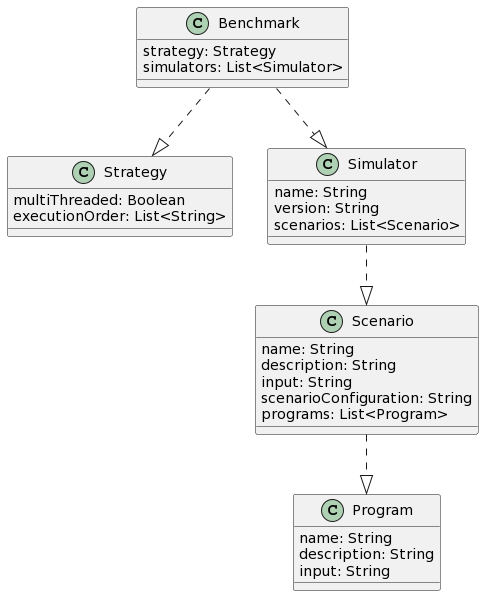
\includegraphics[width=0.7\textwidth]{figures/model.png}
  \caption{Model of the system (v0.1)}
  \label{fig:model}
\end{figure}

As can be seen from the image, the model is 1:1 with the input file.

%----------------------------------------------------------------------------------------
\chapter{Implementation}
%----------------------------------------------------------------------------------------

\section{Technologies}

\subsection{Language}
Different languages were considered for the implementation of the system.

\paragraph*{Scala}
Scala is a strong statically typed high-level general-purpose programming language that supports both object-oriented 
programming and functional programming. 
Designed to be concise, scalable and safe, many of Scala's design decisions are aimed at addressing criticisms of Java.
One weakness of Scala is its steep learning curve, which makes it difficult to learn for new users.

\paragraph*{Kotlin}
Kotlin is a cross-platform, statically typed, general-purpose high-level programming language with type inference. 
Kotlin is designed to interoperate fully with Java.
Support for multiplatform programming is one of Kotlin’s key benefits. It reduces time spent writing and maintaining 
the same code for different platforms while retaining the flexibility and benefits of native programming.
%[https://github.com/JetBrains/kotlin]

\paragraph*{Rust}

Rust is a multi-paradigm programming language designed for performance and safety, especially safe concurrency. \\
It has been designed to be a safe, concurrent, practical language, supporting functional and imperative-procedural paradigms.
It is considered the modern version of C and C++.

\paragraph*{Final choice}
After a brief analysis, it was clear that both Kotlin and Scala were suitable candidates for the implementation of the system.
In the end, the choice fell on Kotlin.

%----------------------------------------------------------------------------------------
\chapter{Conclusion and Future Work}
%----------------------------------------------------------------------------------------

%----------------------------------------------------------------------------------------
% BIBLIOGRAPHY
%----------------------------------------------------------------------------------------

\backmatter

%\nocite{*} % comment this to only show the referenced entries from the .bib file

\bibliographystyle{plain}
\bibliography{bibliography}

\end{document}
